\chapter{Gitárerősítő modellezése}
A félév során az Orange Crush 20L gitárerősítőt modelleztem. Az áramkört az LTSpice segítségével teszteltem. A műveleti erősítőket ideálisnak vettem ott, ahol a valóságnak megfelelő jel esetén nem tapasztaltam levágást, ahol pedig tapasztaltam, ott egy egyszerű levágó algoritmussal modelleztem ezt a jelenséget \cite{opampo}. A frekvenciafüggő átviteltől és a slew rate-től eltekintettem, hiszen modellezésük ilyen komplex rendszer esetén nem fog nagy hangzásbeli különbséget eredményezni.
\begin{figure}[H]
    \centering
    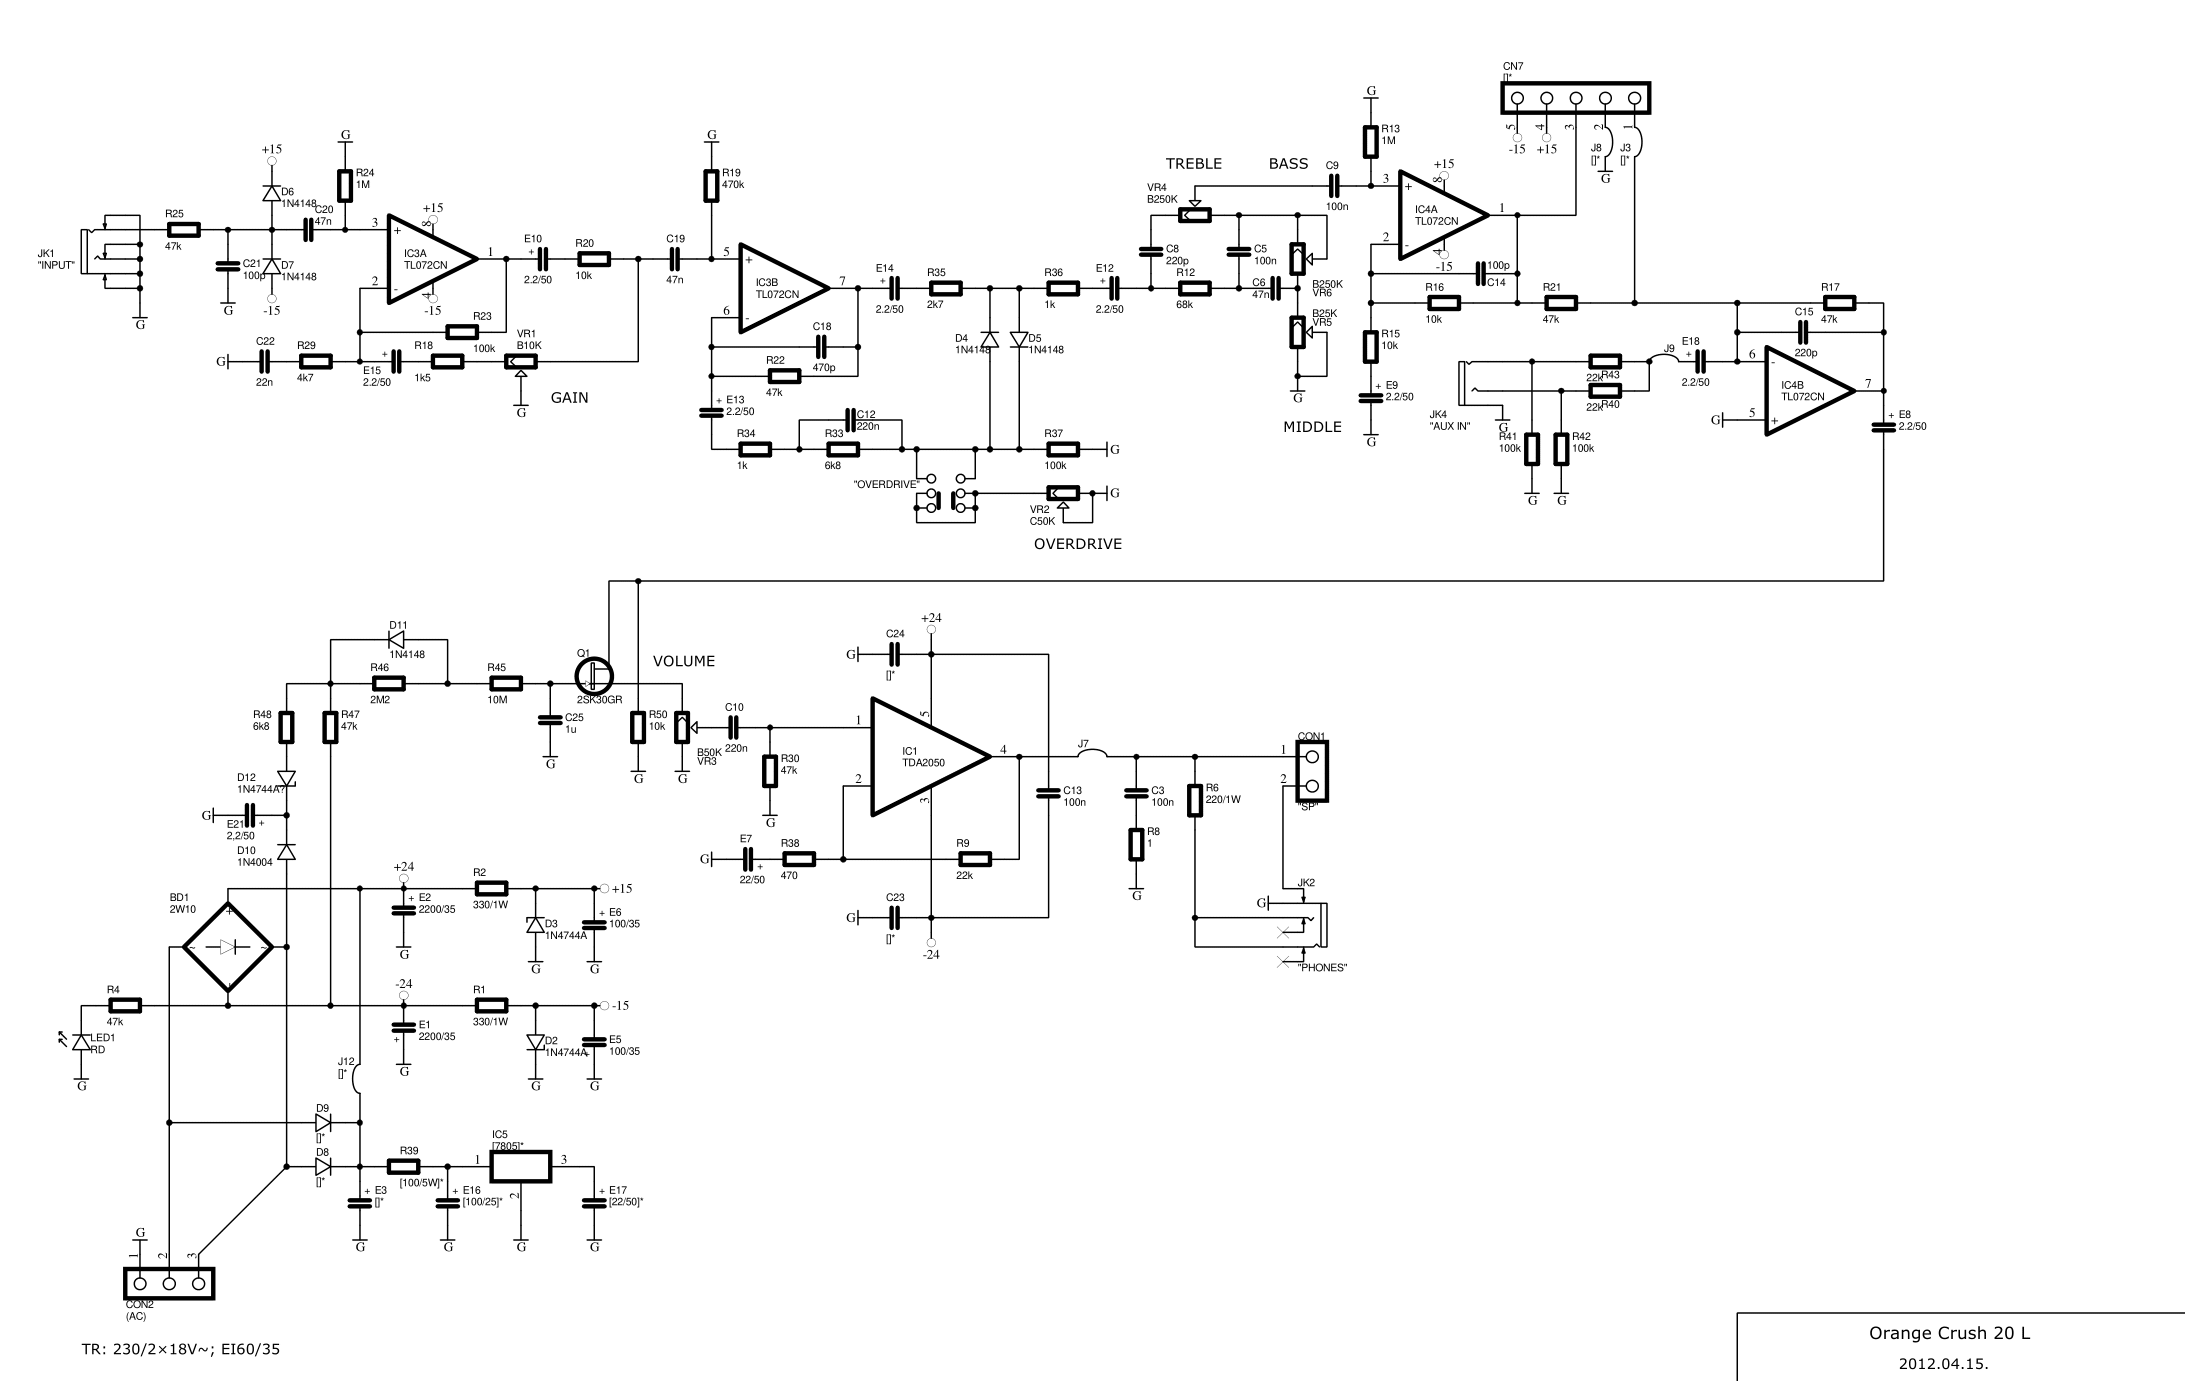
\includegraphics[scale=0.50]{figures/orange_crush_20l_guitar_amp_sch-1.png}
    \caption{Az Orange Crush 20L erősítő áramköre}
\end{figure}

Az áramkört a műveleti erősítők bemeneténél és kimeneténél részekre bontottam, hiszen a műveleti erősítőnek 
nagyimpedanciás bemenete és kisimpedanciás a kimenete, ami miatt az előtte lévő áramköri elemeket nem terheli 
meg, illetve az utána lévő áramkörök nem terhelik meg a műveleti erősítő köré épített részt.
\begin{figure}[H]
    \centering
    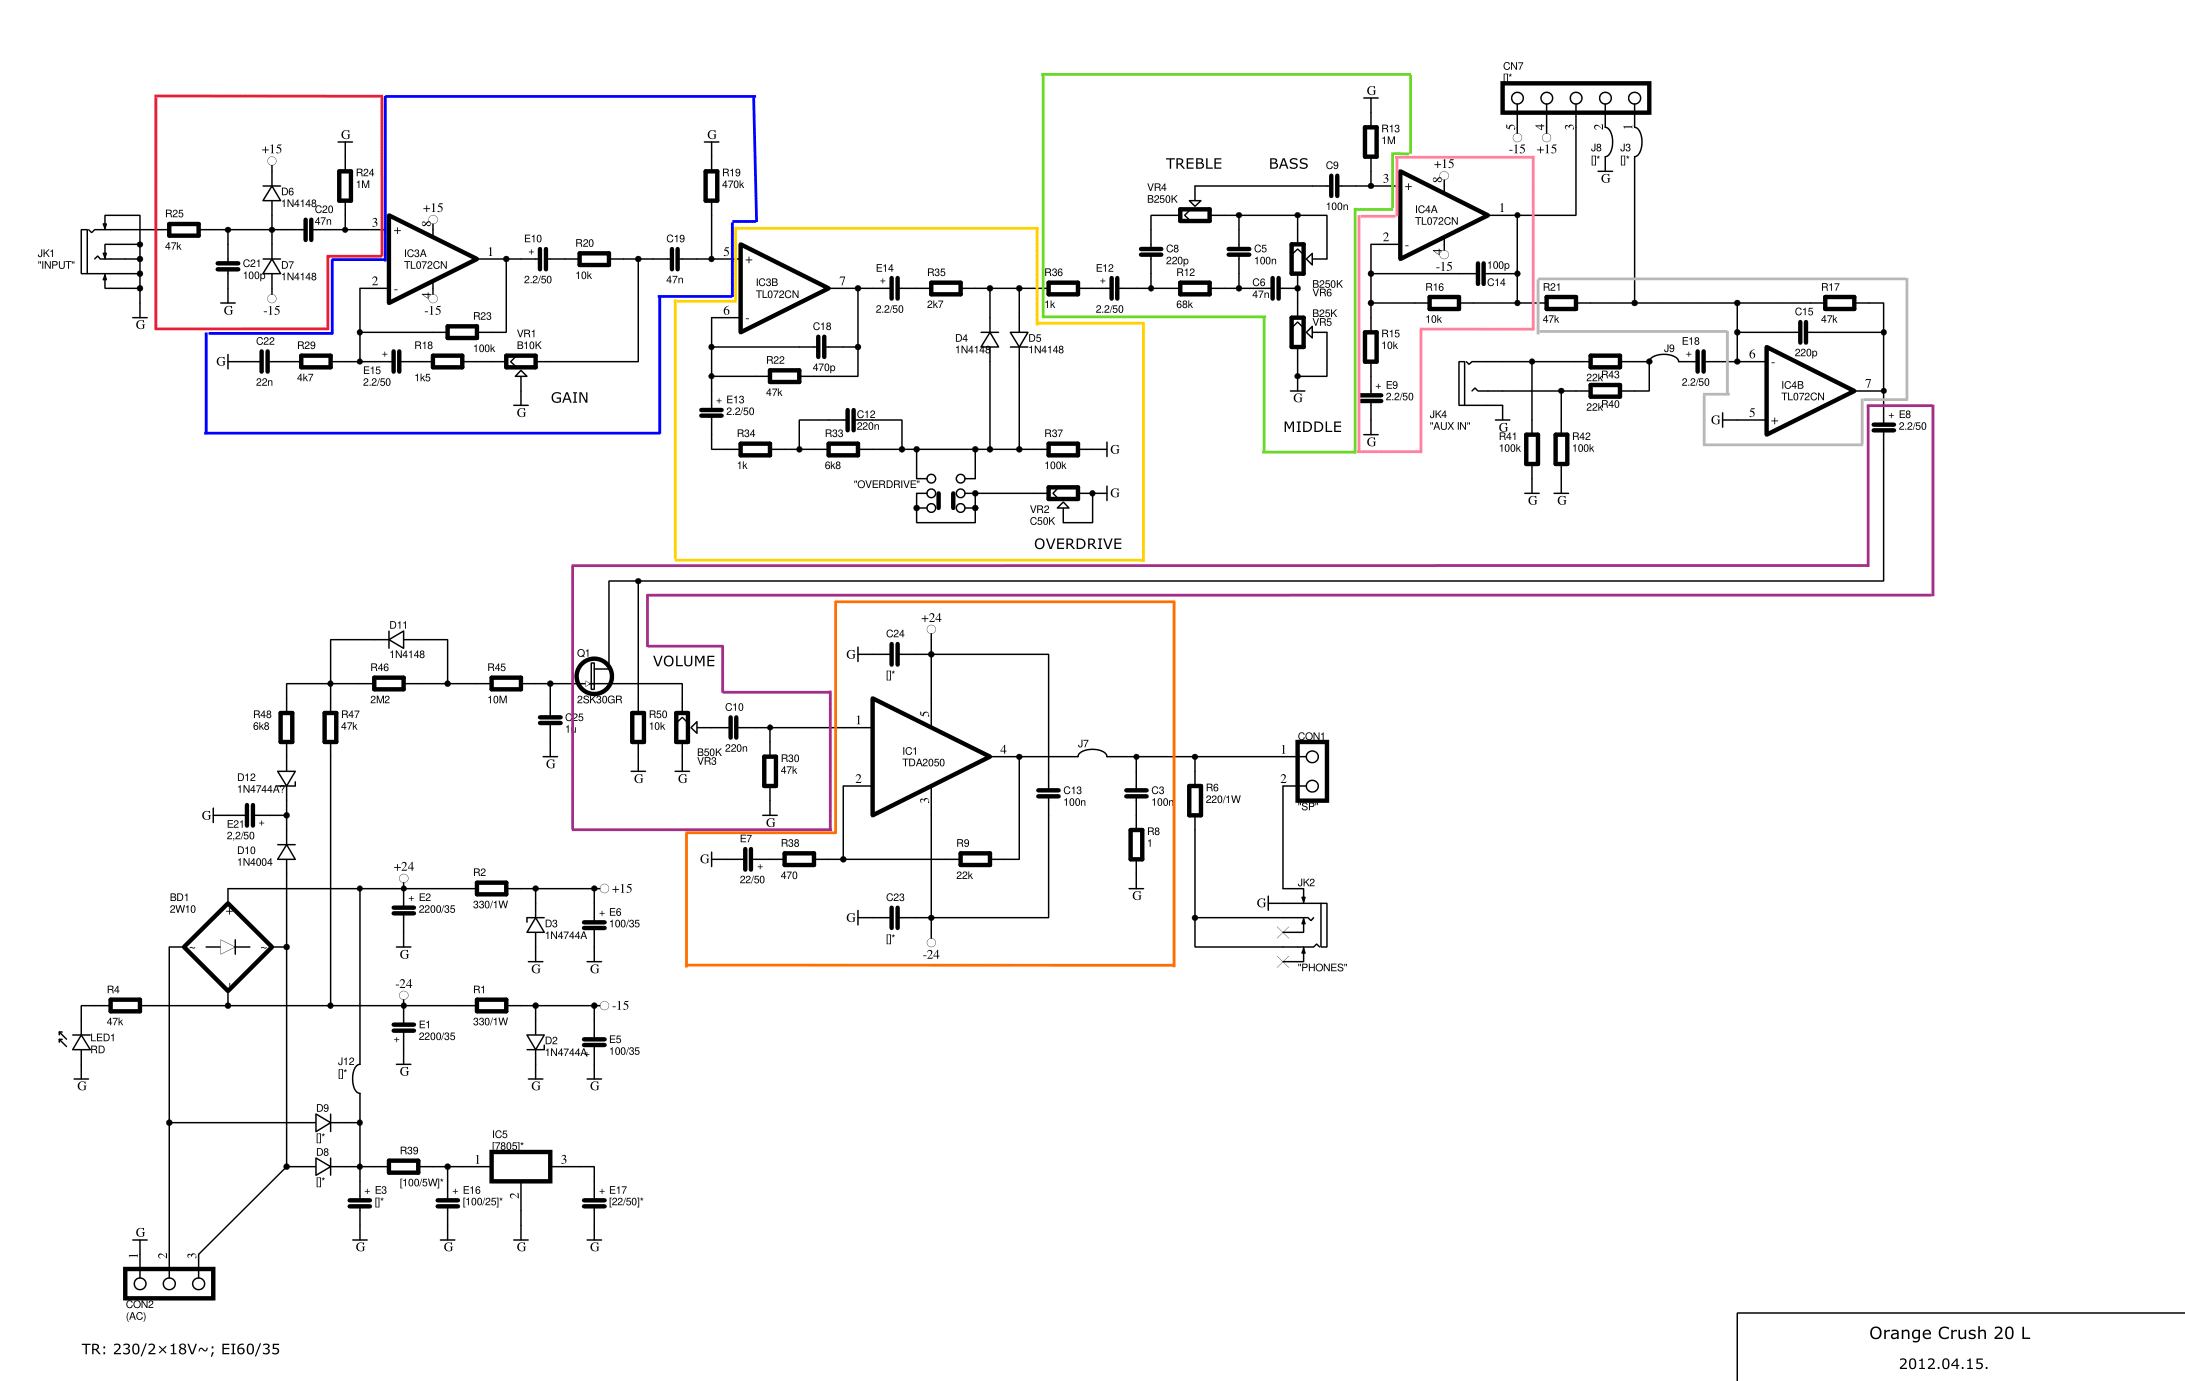
\includegraphics[scale=0.50]{figures/orange_crush_20l_guitar_amp_sch_parts-1.png}
    \caption{Az Orange Crush 20L erősítő áramköre részekre bontva}
\end{figure}
\section{Részáramkörök elemzése}
\subsection{Bemeneti szűrő}

\begin{figure}[H]
    \centering
    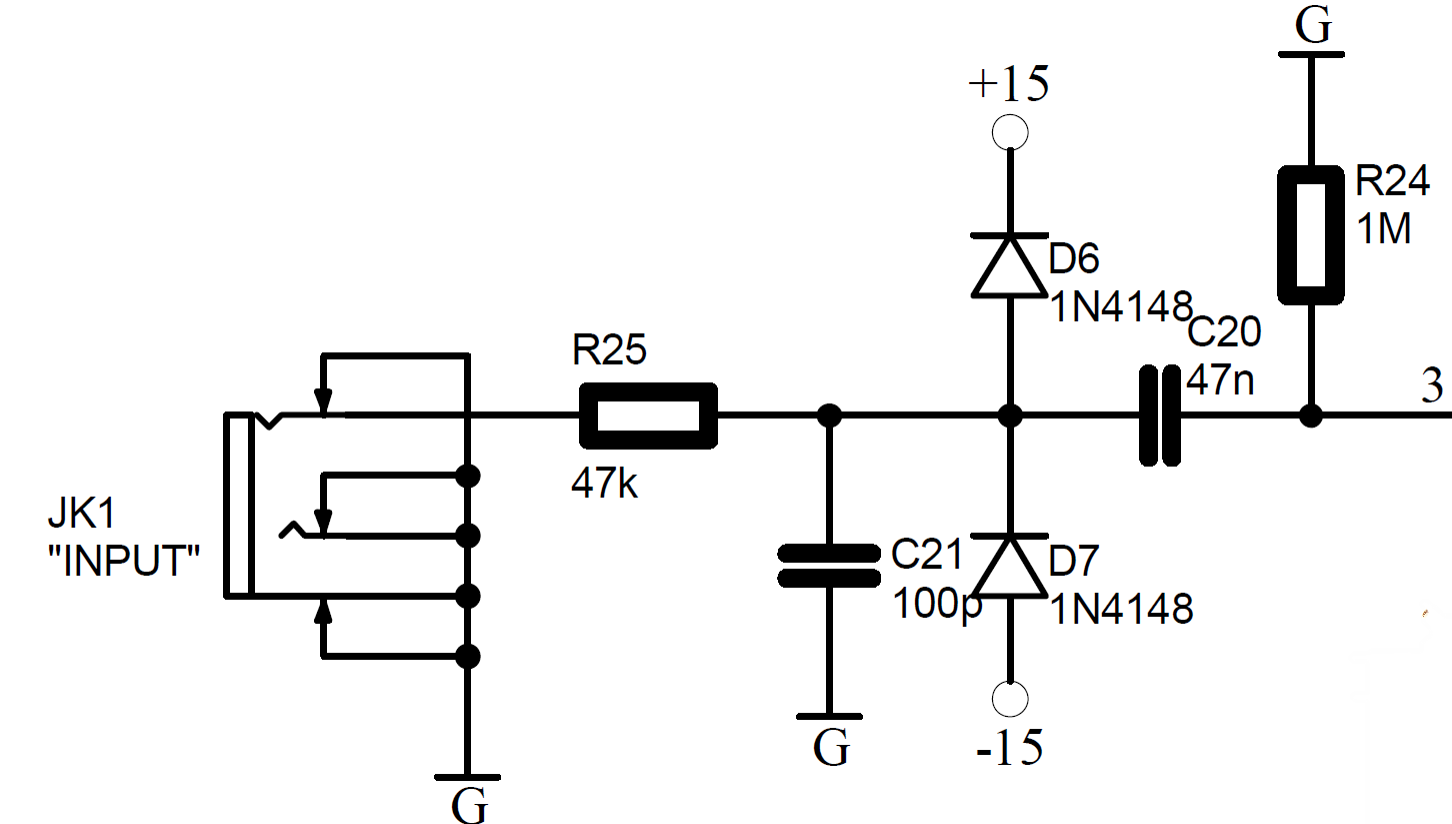
\includegraphics[scale=0.3]{figures/stage1.png}
    \caption{A bemeneti szűrők}
\end{figure}

A bemeneti szűrő egy alul- és egy felüláteresztő RC szűrőből áll. A diódák csak védelem miatt vannak, hogy a 
műveleti erősítő bemenetére ne kerüljön semmiféle módon több feszültség, mint a tápfeszültsége, ezért a 
modellezésben elhanyagolhatjuk.

A hálózatot bilineáris transzformációval modellezve az alábbi eredményeket kaptam az LTSpice szimulációval összehasonlítva:
\begin{figure}[H]
    \centering
    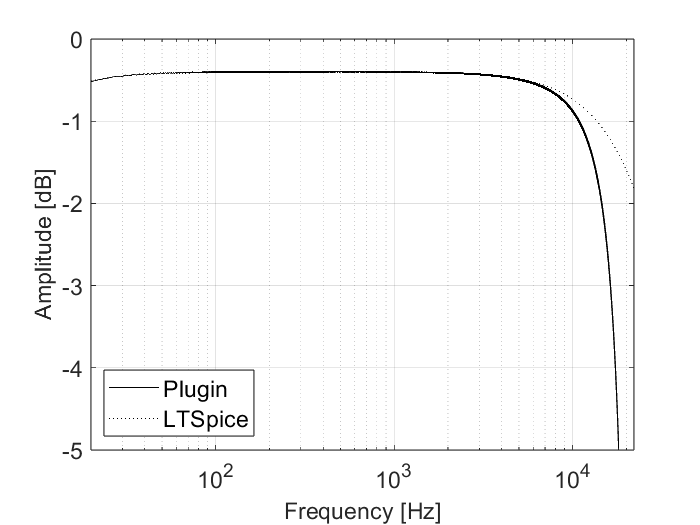
\includegraphics[scale=0.5]{figures/stage1plot.png}
    \caption{Az LTSpice szimuláció eredménye összehasonlítva a megvalósított szűrővel}
\end{figure}

A különbség a bilineáris transzformációnak köszönhető, hiszen egy bilineárisan transzformáció segítségével létrehozott 
diszkrét idejű rendszer a mintavételi frekvenciához 
közeli frekvenciákon jelentősen el tud térni az eredeti folytonos idejű rendszertől. 
Mint látható, hogy a frekvenciamenetek megegyeznek körülbelül $6kHz$-ig, 
és a $6dB$ különbséget pedig jóval $18kHz$ után éri el.

\section{Erősítő rész}
\begin{figure}[H]
    \centering
    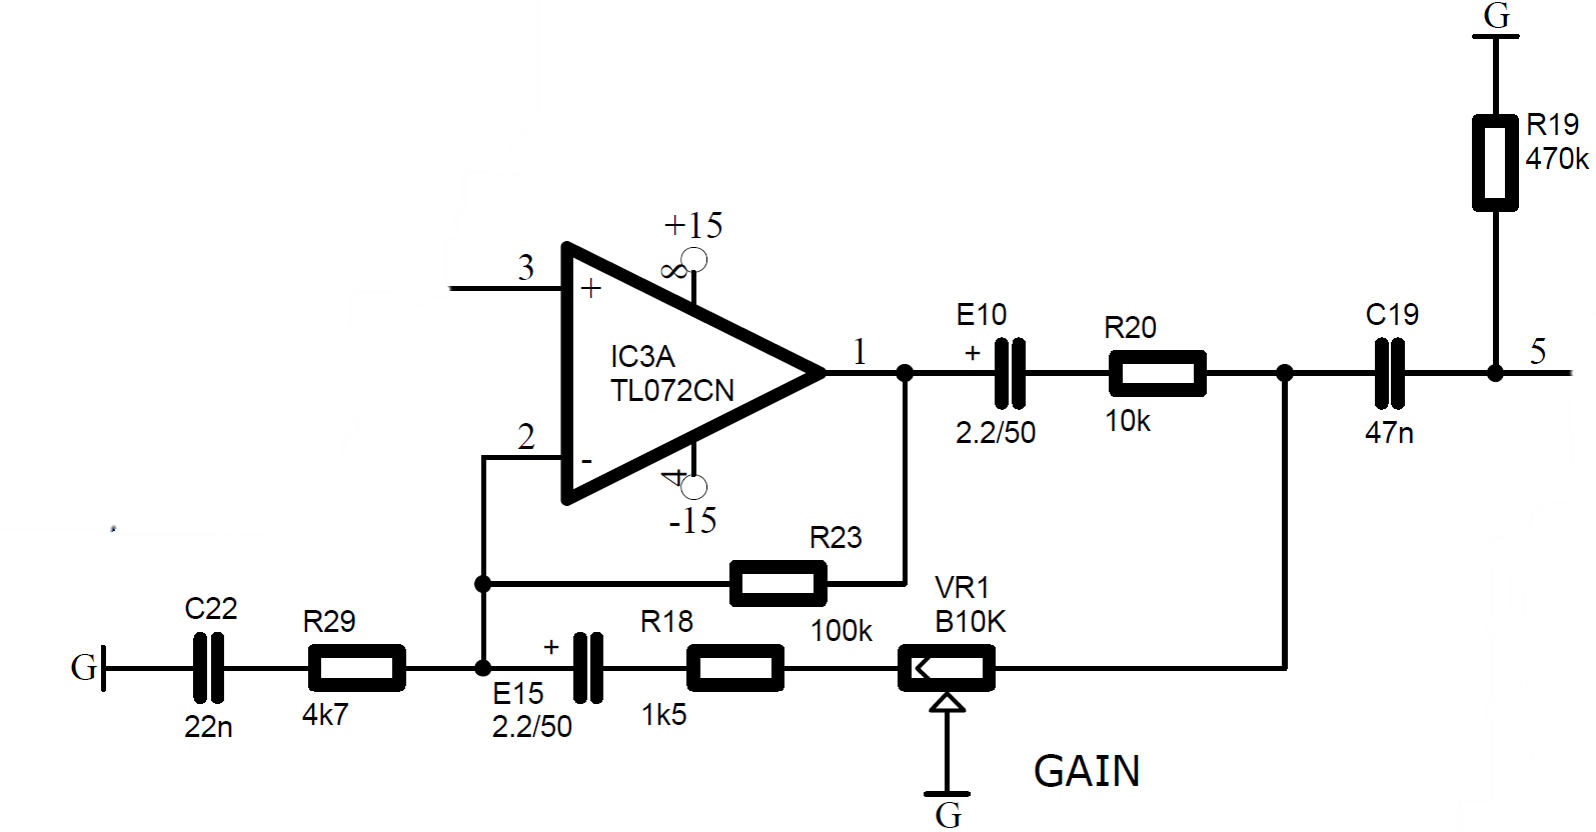
\includegraphics[scale=0.35]{figures/stage2.png}
    \caption{A bemeneti szűrők}
\end{figure}
Az erősítő kimeneténél felbontottam az áramkört (az $1$ pontnál), először a műveleti erősítőt tartalmazó részt 
modelleztem, utána pedig a passzív hálózatot. Mind a két részt bilineáris transzformáció segítségével modelleztem. 

LTSpice szimuláció segítségével észrevettem, hogy a valóságnak megfelelő bemeneti jel esetén is a 
GAIN potméter adott állásaiban le fog vágni a műveleti erősítő a tápfeszültségénél. 

\begin{figure}[H]
    \centering
    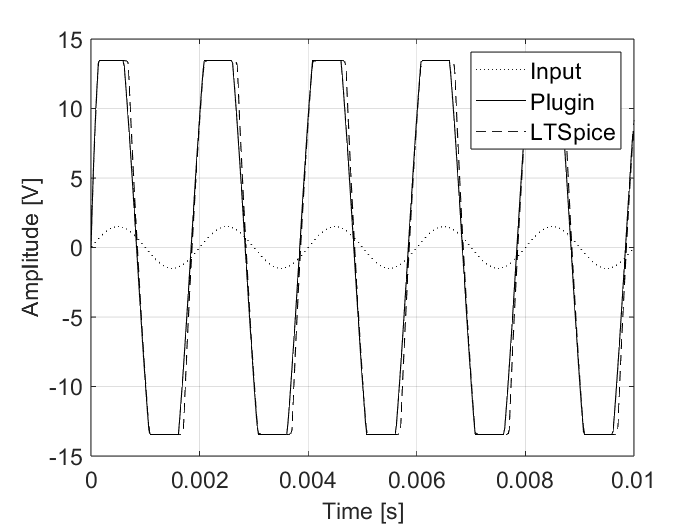
\includegraphics[scale=0.5]{figures/stage2plot.png}
    \caption{A műveleti erősítő válasza egy $500Hz$-es $1.5V$ amplitúdós szinusz jelre}
    \label{again}
\end{figure}

A (\ref{again}) ábrán lehet látni a jelalak minimálisan eltérését az LTSpice szimuláció eredményétől. 
Ez annak köszönhető, hogy az LTSpice-ban lévő műveleti erősítő modell a műveleti erősítő frekvenciafüggését és slew 
rate-jét is figyelembe veszi, illetve valószínűleg sokkal bonyolultabb karakterisztikát használ.

A műveleti erősítő levágását egyszerű levágó algoritmussal valósítottam meg \cite{opampo} \cite{opamp}. Eredetileg az ideális műveleti erősítőt tartalmazó modell fut, és ha annak a kimenete túllépné az LTSpice alapján meghatározott levágási feszültséget, akkor a szarutációs modellel visszaszámolom a bemenetet (ekkor a kimenete a levágási feszültség). A rendszeregyenlet segítségével egyszerűen visszaszámolható a bemenet, azt csak át kell rendezni $u[n]$-re, $y[n]$ adott. Ezután a bufferekben ezek alapján kell frissíteni az értékeket.
\begin{figure}[H]
    \centering
    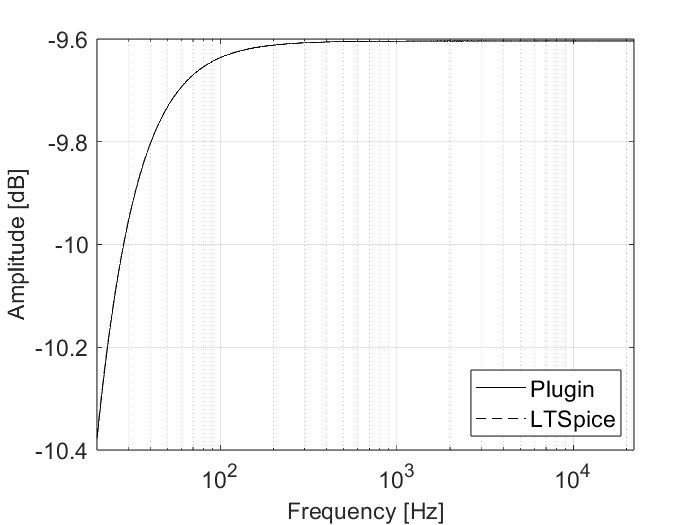
\includegraphics[scale=0.5]{figures/stage2after.png}
    \caption{A műveleti erősítő utáni passzív hálózat tesztelése. A GAIN potméter $5k\Omega$ értékre volt állítva.}
\end{figure}
A passzív hálózat felüláteresztő jellege miatt a bilineáris transzformációval létrehozott modell jól követi a frekvenciamenetet. 

\section{Torzító rész}
\begin{figure}[H]
    \centering
    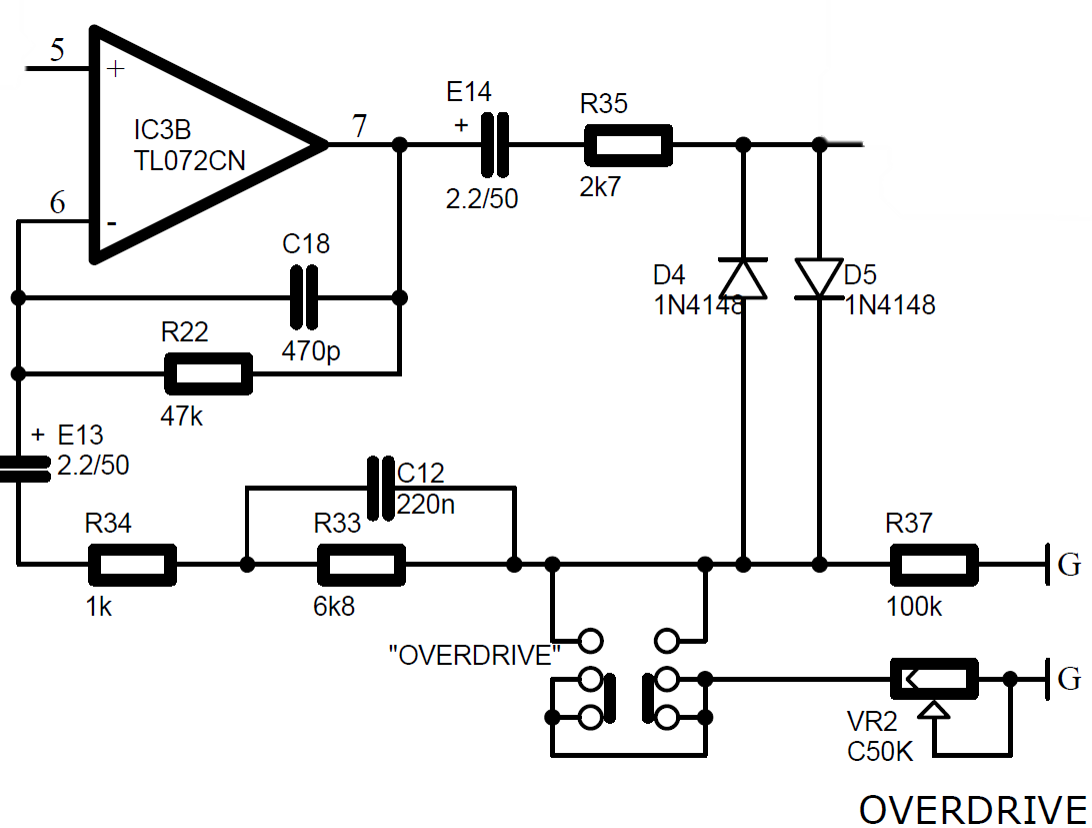
\includegraphics[scale=0.35]{figures/stage3.png}
    \caption{A torzító rész áramköre}
\end{figure}

A torzító rész utáni áramkörrészt leválasztottam, és különböző részként kezeltem. Ezt azért tehettem meg, mert annak a bemeneti impedanciája sokkal nagyobb, mint a torzító rész kimeneti impedanciája, azaz a torzító rész feszültséggenerátorosan hajtja meg az utána következő részeket (ezt LTSpice-ban egy követő erősítő segítségével is teszteltem).
\begin{figure}[H]
    \centering
    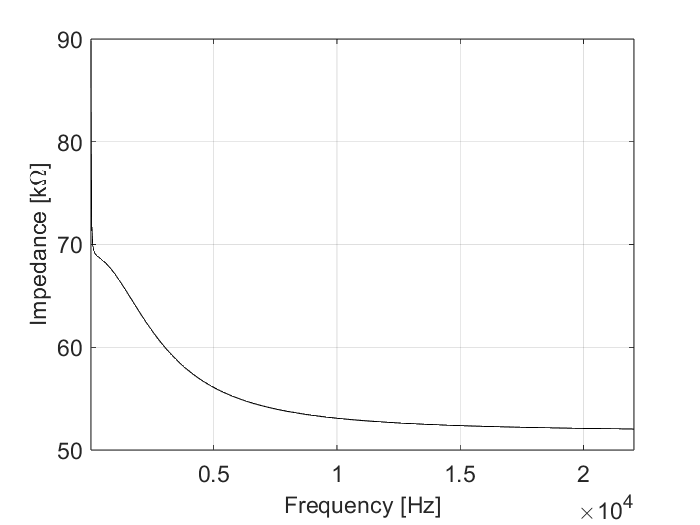
\includegraphics[scale=0.5]{figures/res.png}
    \caption{A torzító részt követő áramkör bemeneti impedanciája}
\end{figure}

A torzító rész modellezéséhez K-módszert használtam, ahol a diódák okozták a nemlinearitást. Tesztelés céljából a táblázatot az általános $i(u)=I_{S0}(1-e^{-\frac{u}{u_T}})$ függvény alapján generáltam le. Ha csak a diódákat vettem bele a nemlineáris függvénybe, akkor nem tudtam kifejezni a kimenetet (hasonló probléma jelenik meg egy feszültségforrásra sorosan kötött dióda és ellenállásnál). A problémát azzal oldottam meg, hogy az $R_{35}$ soros ellenállást is beleszámoltam a nemlineáris függvénybe, és így hoztam létre a táblázatot. Az áramra egy implicit egyenlet jött ki, a feszültségre egy explicit, így a feszültség alapján generáltam le a táblázatot.
\pagebreak
\begin{equation}
    f(u)=i=I_{S0}sinh(\frac{u-R_{35}i}{u_T})
\end{equation}
\begin{equation}
    f^{-1}(i)=u=u_Tsinh(\frac{i}{2I_{S0}})+R_{35}i
\end{equation}
Ezután kiexprotáltam a karakterisztikát ismét LTSpice-ból, és végül ezt használtam majd a végleges eredményhez.

Az LTSpice szimuláció során észrevettem, hogy a műveleti erősítő kimenetén olyan feszültségszintek fordulhatnak elő valósághű bemenetek esetén, amelyeknél meghatározó lesz a műveleti erősítő tápfeszültségének szintje, és le fogja vágni, ha afelé menne. Ennek a modellezése már nem fért bele az Önálló laboratórium tárgyba, viszont egy jó ötlet továbbfejlesztési lehetőségnek. Erre a megoldás egy egyszerű levágó algoritmus lenne \cite{opampo} \cite{opamp}. Az ideális modellel kiszámolnám a műveleti erősítőnknek a kimenetén lévő feszültséget, és ha ez meghaladja a tápfeszültséget, akkor a kimenetére megszabom, abból a bemenetet visszaszámolom, és ez alapján futtatni a K-módszer algoritmusát.\\
Az állapotváltozós leírás alapján kiszámolt mátrixok:
\begin{equation}
    \begin{array}{c}
        \mathbf{A}=
        \begin{pmatrix}
            -\frac{1}{C_{12}(R_{37}+R_{34})}-\frac{1}{C_{12}R_{33}} & 0 & -\frac{1}{C_{12}(R_{37}+R_{34})} & 0 \\
            \frac{1}{C_{18}(R_{37}+R_{34})} & -\frac{1}{R_{22}C_{18}} & \frac{1}{C_{18}(R_{37}+R_{34})} & 0 \\
            -\frac{1}{E_{13}(R_{37}+R_{34})} & 0 & -\frac{1}{E_{13}(R_{37}+R_{34})} & 0 \\
            0 & 0 & 0 & 0
        \end{pmatrix} \\ \\
        \mathbf{B}=
        \begin{pmatrix}
            -\frac{1}{C_{12}(R_{37}+R_{34})} \\
            \frac{1}{C_{18}(R_{37}+R_{34})} \\
            -\frac{1}{E_{13}(R_{37}+R_{34})} \\
            0
        \end{pmatrix} \qquad
        \mathbf{C}=
        \begin{pmatrix}
            \frac{R_{37}}{C_{12}(R_{37}+R_{34})} \\
            1 \\
            -\frac{R_{37}}{R_{37}+R_{34}} \\
            1
        \end{pmatrix} \\ \\
        \mathbf{D}=
        \begin{pmatrix}
            -\frac{R_{37}}{R_{37}+R_{34}} & 1 & -\frac{R_{37}}{R_{37}+R_{34}} & 1 
        \end{pmatrix} \qquad
        E=\frac{R_{34}}{R_{37}+R_{34}} \qquad
        F=-\frac{R_{34}R_{37}}{R_{37}+R_{34}}
    \end{array}
\end{equation}
A (\ref{G}), (\ref{H}), (\ref{J}), (\ref{K}) egyenletekkel kiszámoltam a segédváltozókat, és a (\ref{iter}) lépései szerint programoztam be az algoritmust.Az általam számolt karakterisztikával kapott eredmény a (\ref{nospicenoclip}) és a (\ref{nospiceclip}) ábrán, az LTSpice-ból kiexportált karakterisztikával kapott eredmények pedig a (\ref{spicenoclip}) és (\ref{spiceclip}) ábrán látható.
\begin{figure}[H]
    \centering
    \begin{subfigure}{0.47\textwidth}
        \centering
        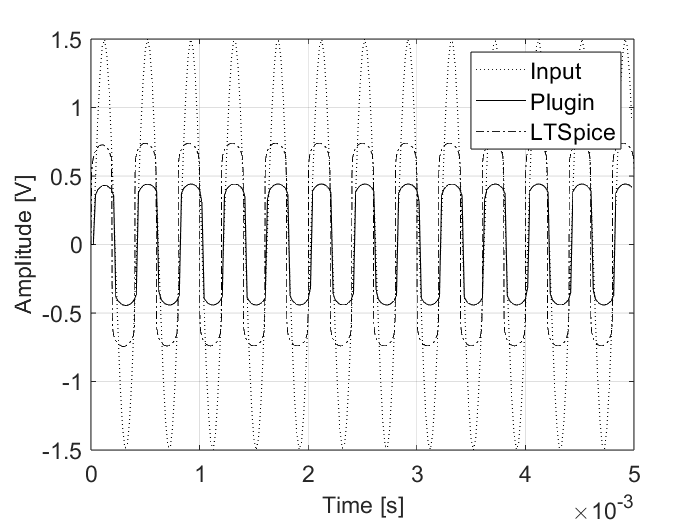
\includegraphics[scale=0.38]{figures/nospicenoclip.png}
        \caption{}
        \label{nospicenoclip}
    \end{subfigure}
    \hfill
    \begin{subfigure}{0.47\textwidth}
        \centering
        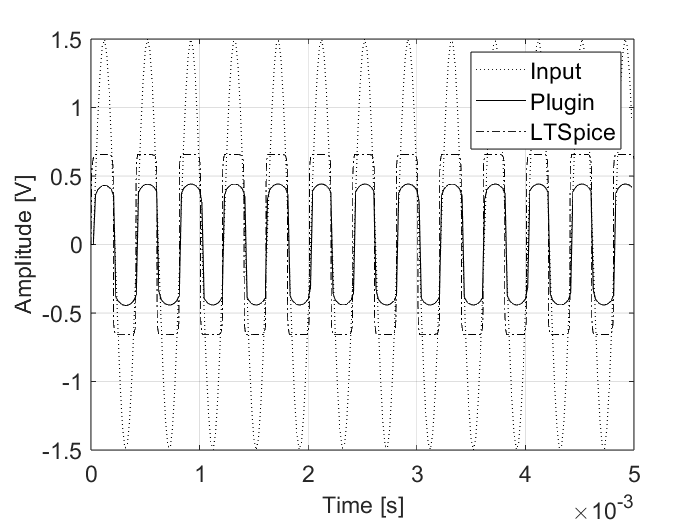
\includegraphics[scale=0.38]{figures/nospiceclip.png}
        \caption{}
        \label{nospiceclip}
    \end{subfigure}
    \begin{subfigure}{0.47\textwidth}
        \centering
        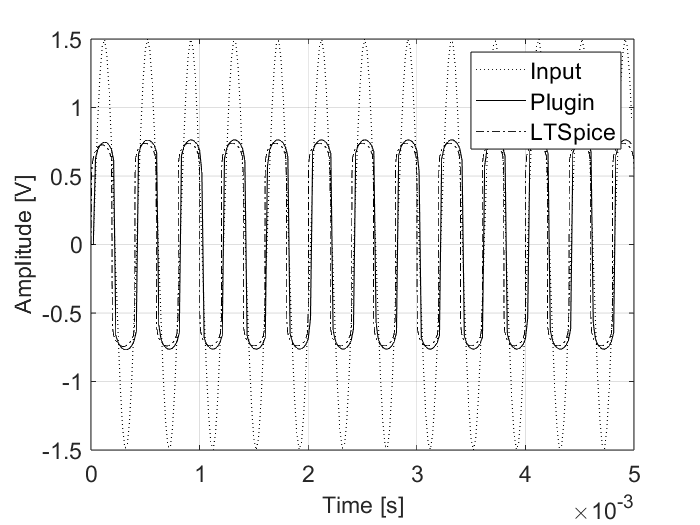
\includegraphics[scale=0.38]{figures/spicenoclip.png}
        \caption{}
        \label{spicenoclip}
    \end{subfigure}
    \hfill
    \begin{subfigure}{0.47\textwidth}
        \centering
        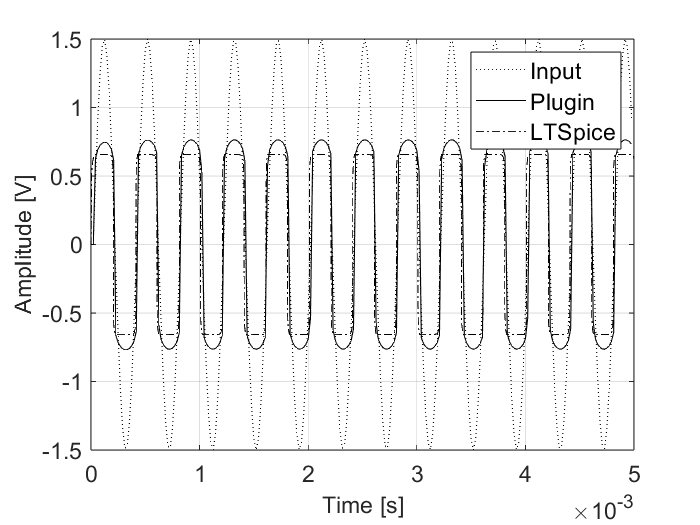
\includegraphics[scale=0.38]{figures/spiceclip.png}
        \caption{}
        \label{spiceclip}
    \end{subfigure}
    \caption{A plugin és az LTSpice által adott válasz, (\ref{nospicenoclip}) és (\ref{spicenoclip}) ábrán amikor az LTSpice-ban ideális műveleti erősítőt használok, és (\ref{nospiceclip}) és (\ref{spiceclip}) ábrán amikor a nem ideális műveleti erősítő modellt használok}
\end{figure}
A megvalósítás során nehézséget okozott az OVERDRIVE paraméter, hiszen minden egyes változásánál változni fognak a segédváltozóink, azaz minden egyes paraméterváltozásnál újra ki kell számolnunk a (\ref{G}), (\ref{H}), (\ref{J}), (\ref{K}) egyenleteket, majd el kell végezni az $f(u)$ függényünkre a lineáris interpolációt (hiszen függ $K$ értékétől). Természetesen amikor a (\ref{iter}) egyenletrendszer lefut, mindig ki lehetne ezt a transzformációt számolni, de egyáltalán nem célszerű. Ezt a problémát a JUCE környezet $juce::AudioProcessorValueTreeState::Listener$ osztályából való örökléssel oldottam meg. Ennek az osztálynak van egy \textit{void parameterChanged(const juce::String\& parameterID, float newValue)} nevű függvénye, ami mindig csak akkor hívódik meg, amikor a hozzá tartozó paraméter értéke változik.
\section{Tone stack}
\begin{figure}[H]
    \centering
    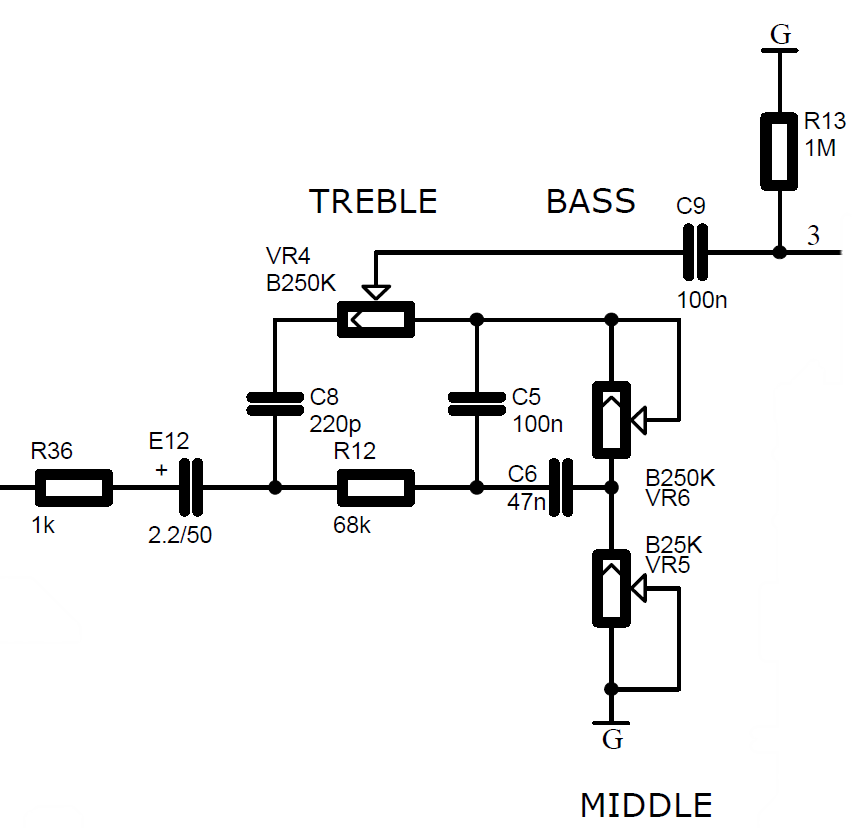
\includegraphics[scale=0.35]{figures/stage4.png}
    \caption{Az erősítő tone stack áramköre}
\end{figure}
Az erősítő tone stack részét is szintén bilineáris transzformáció segítségével modelleztem. Sok nehézséget okozott a sok paraméter (itt három is van, $BASS$, $MID$, $TREBLE$, ráadásul a mintavételi idő is), illetve az, hogy a transzformáció során kiszámolandó értékek számára nem adott elég nagy pontosságot a $float$ típus, emiatt $double$ típust kellett használnom. A transzformált rendszer néhány pólusa olyan közel voltak az egységkörhöz, hogy a potméterek bizonyos állásainál a legközelebbi pólus az egységkörön kívülre esett. Ezt a $double$ típusban való tárolás megoldotta. 

A tone stack rész paraméteres felírása és beprogramozása nagyon körülményes feladat, így ez most nem került megvalósításra, de mindenképpen egy továbbfejlesztési lehetőség.
\section{Aktív szűrő}
\begin{figure}[H]
    \centering
    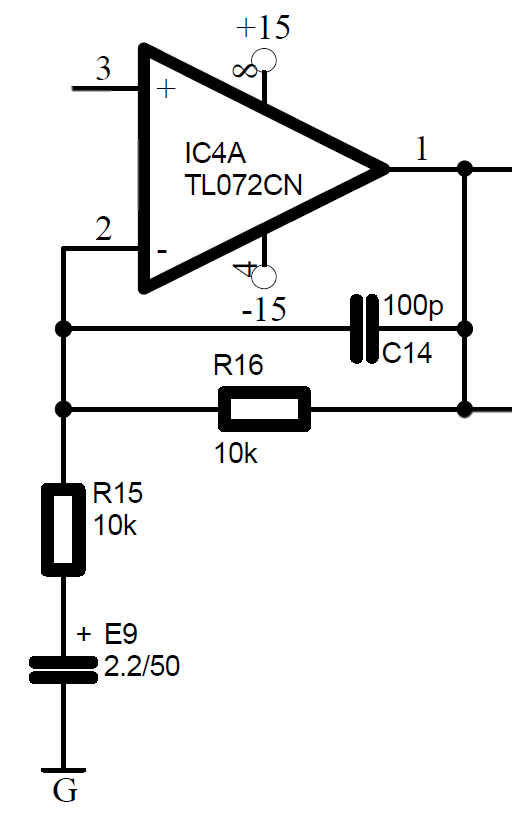
\includegraphics[scale=0.35]{figures/stage5.png}
    \caption{Az erősítő tone stack után lévő aktív szűrő áramkör}
\end{figure}
Egyszerű aktív szűrő, bilineáris transzformáció segítségével modelleztem. Célja az áramkörben, hogy az esetleges mély- és magas frekvenciakomponenseket kiszűrje. A bilineáris transzformáció miatt a mintavételi frekvenciákhoz közeli frekvenciákon nem pontos, hiszen bilineáris transzformáció segítségével modellezett diszkrét rendszer átvitele jelentősen eltérhet az eredeti folytonos idejű rendszer átvitelétől a mintavételi frekvencia közelében.
\begin{figure}[H]
    \centering
    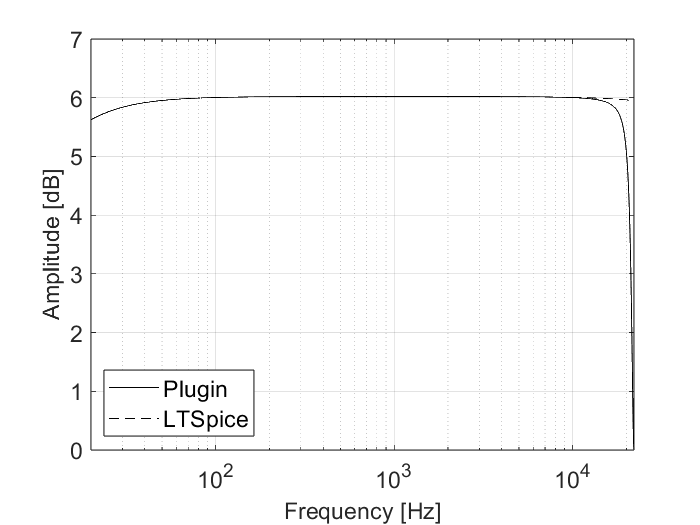
\includegraphics[scale=0.5]{figures/stage5ac.png}
    \caption{Az erősítő tone stack után lévő aktív szűrő áramkörének a modellezett átvitele az eredeti átvitelhez képest}
\end{figure}

\section{Összeadó áramkör}
\begin{figure}[H]
    \centering
    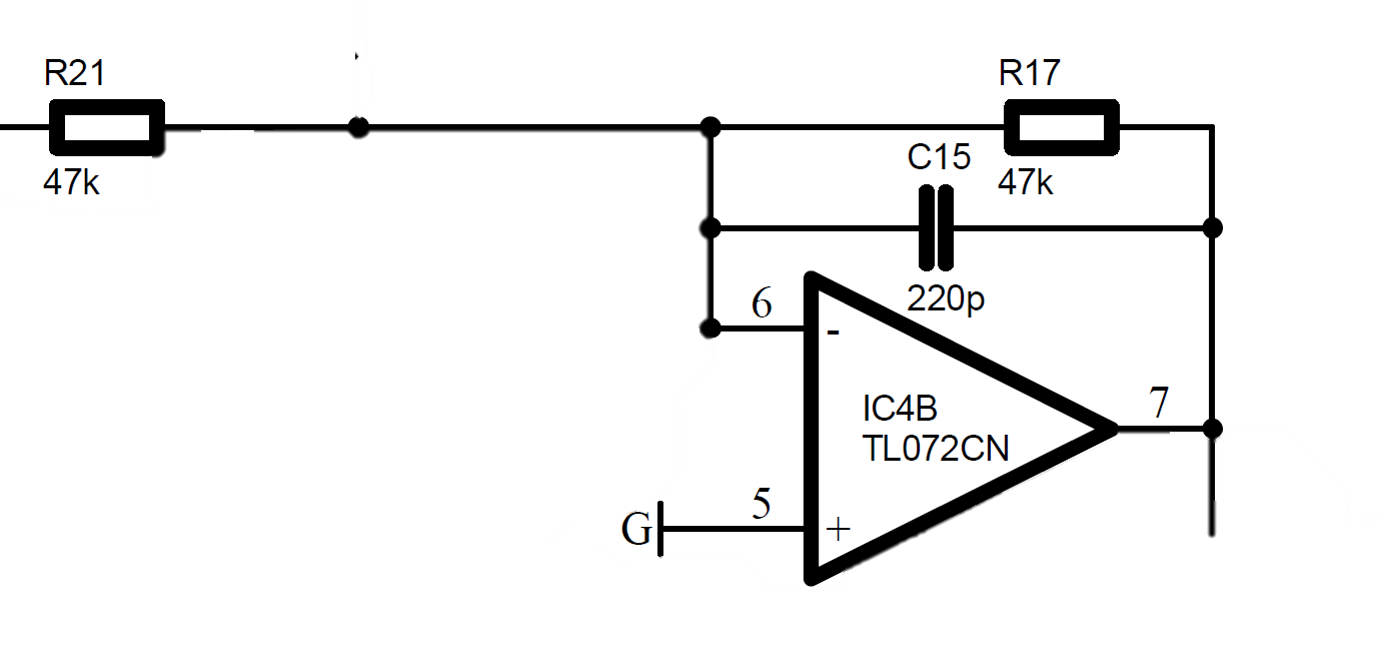
\includegraphics[scale=0.35]{figures/stage6.png}
    \caption{Az áramkör, ami az erősítő jack bemenetén beadott jelet összeadja az erősítő jelével}
\end{figure}

Ez az áramköri rész azért felel, hogy az erősítőbe jack csatlakozón beadott jelet összeadja az erősítő jelével. Mivel a jack csatlakozón beadott jelet nem akarjuk módosítani, ezért minden hangszínváltoztatás és torzítás után van ez az áramkör. Az erősítése egységnyi, és egy aluláteresztő szűrőt valósít meg, hogy a jack bemenetről bejövő nagy frekvenciájú komponenseket kiszűrje. Bilineáris transzformáció segítségével modelleztem.
\begin{figure}[H]
    \centering
    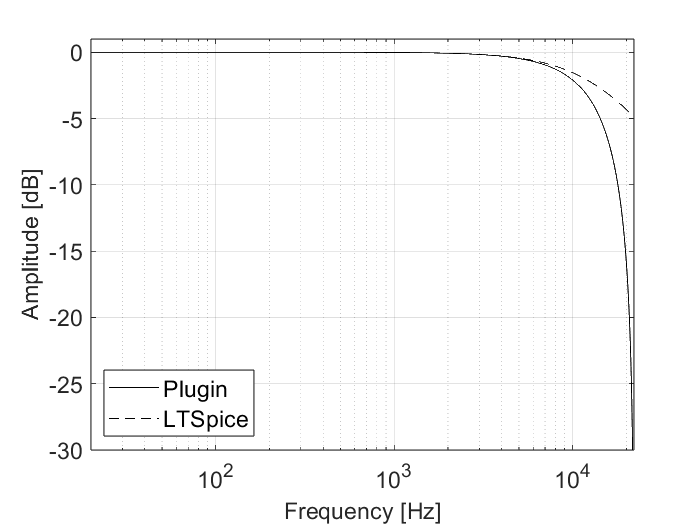
\includegraphics[scale=0.5]{figures/stage6ac2.png}
    \caption{Az áramkör, ami az erősítő jack bemenetén beadott jelet összeadja a gitár jelével}
\end{figure}

\section{Hangerőszabályozó}

\begin{figure}[H]
    \centering
    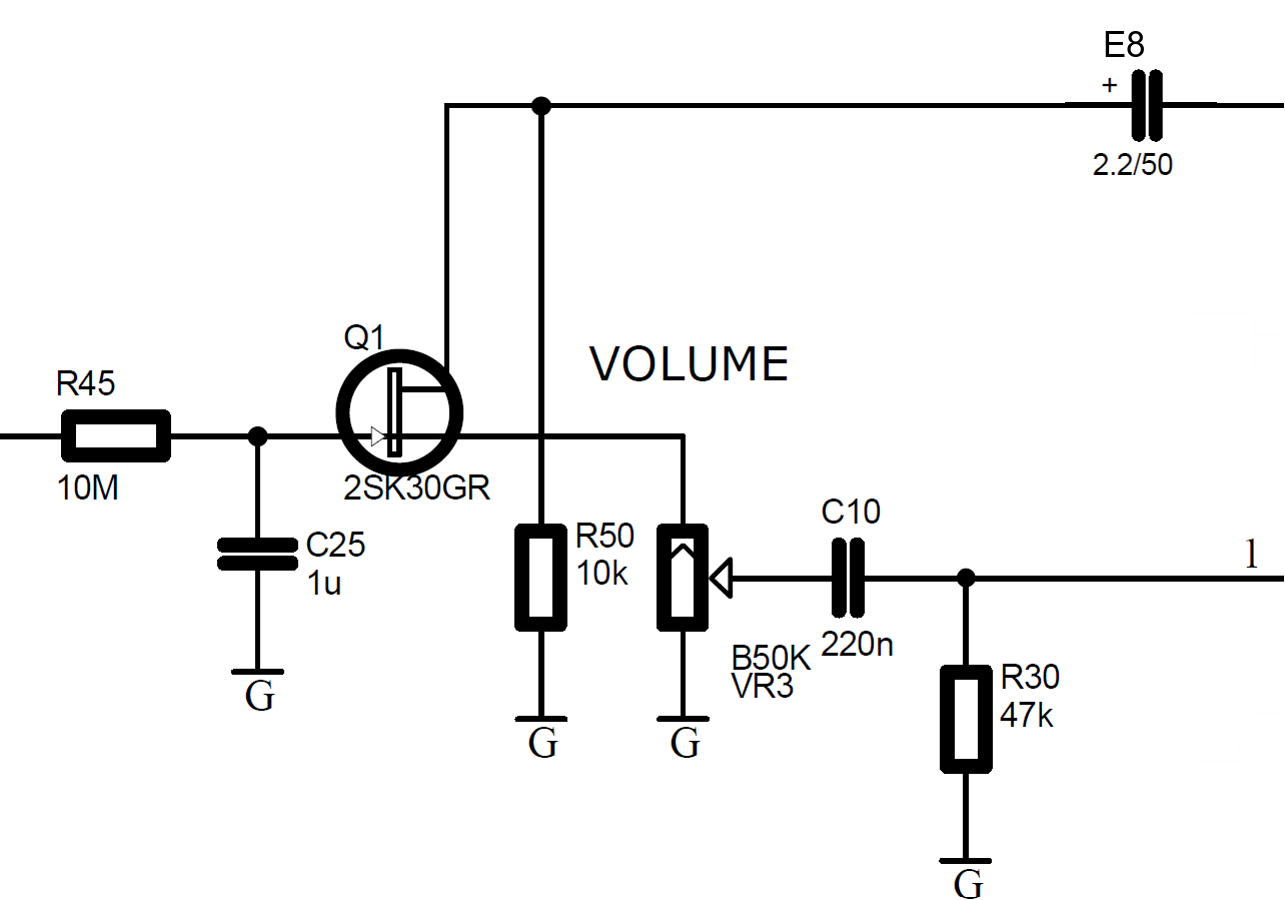
\includegraphics[scale=0.45]{figures/stage7.png}
    \caption{Az erősítő hangerőszabályzó áramköre}
\end{figure}

Az eredeti áramkörben lehet látni egy MOSFET tranzisztort a hangerőszabályzó potméter előtt. Ez a tranzisztor a végfokozat védelmét biztosítja. A MOSFET gate elektródáján lévő $1\mu F$ kapacitású kondenzátor lassan fog feltöltődni az előtte található $10M\Omega$-os ellenálláson. Miután feltöltődött teljesen, utána a MOSFET gate-jén konstans feszültség lesz, nyitva lesz, és az impedanciája az alapján fog változni, amennyi feszültség esik rajta, viszont ez $m\Omega$ nagyságrendekben lesz, ami elhanyagolható az utána lévő $10k\Omega$-os osztó miatt.

A részáramkört szintén bilineáris transzformáció segítségével modelleztem.

\begin{figure}[H]
    \centering
    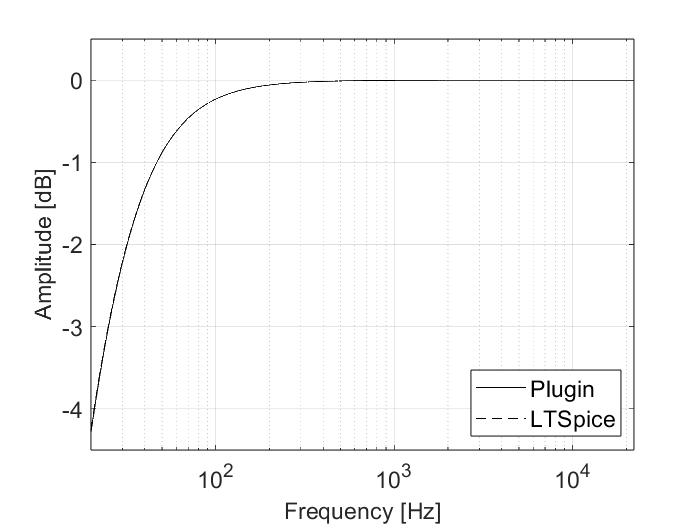
\includegraphics[scale=0.5]{figures/stage7ac3.png}
    \caption{A részáramkör átvitele a VOLUME potméter maximum értéke, azaz $10k\Omega$ mellett}
\end{figure}


\section{Végfokozat}
\begin{figure}[H]
    \centering
    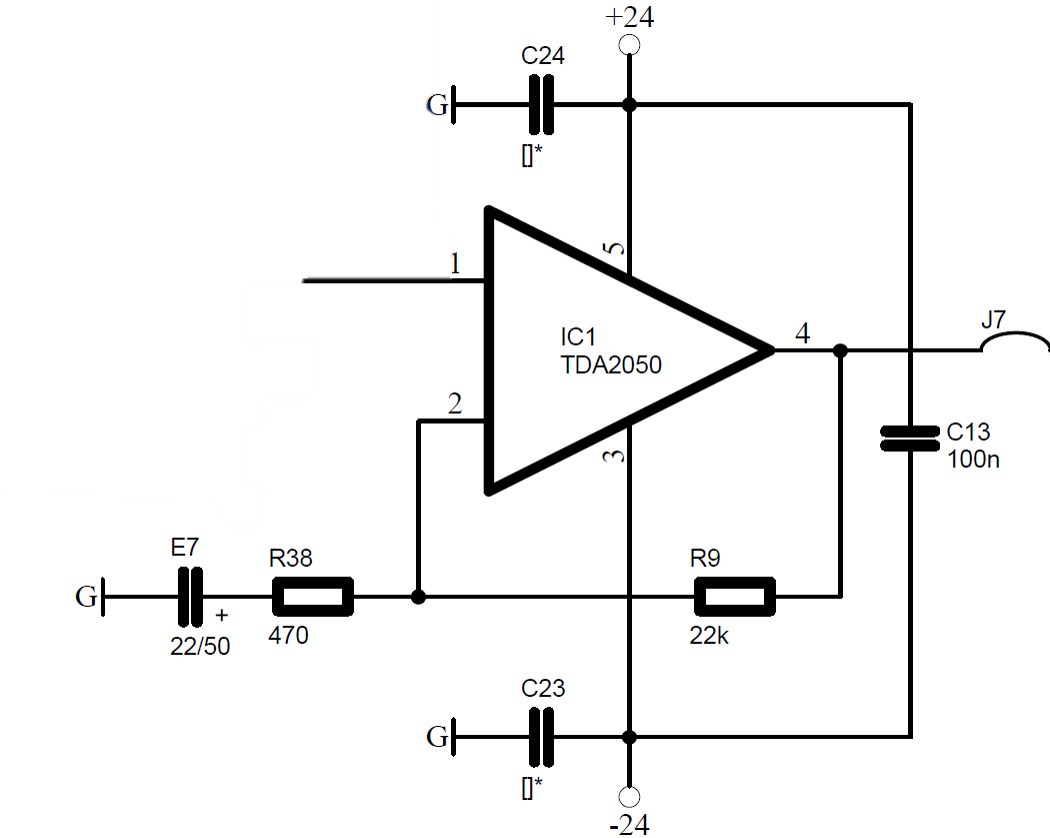
\includegraphics[scale=0.35]{figures/stage8.png}
    \caption{Az erősítő kimenő fokozatának áramköre}
\end{figure}
Ez az áramköri rész gondoskodik arról, hogy az erősítő jelét felerősítse olyan szintre, hogy ezután már csak a hangszóróra kelljen rávezetni. A műveleti erősítő tápján a kondenzátoroknak a tápfeszültség stabilitása a célja, hogy mind a közös módusú, mind pedig a differenciál módusú zavarok ellen védelmet nyújtsanak. Az $E7$ kondenzátornak köszönhetően az átvitelnek felüláteresztő jellege lesz.Ezt az áramköri részt is bilineáris transzformáció segítségével modelleztem. A műveleti erősítő a folytonos idejű áramkörnél levág nagyobb hangerőszinteknél, ez viszont valószínűleg nem cél. Ennek ellenére megvalósítottam ezt is egy egyszerű levágó algoritmussal \cite{opampo}, hogy könnyebben tudjam a plugin hangerőszintjeit skálázni (megfelelő legyen digitális szinteknek).
\begin{figure}[H]
    \centering
    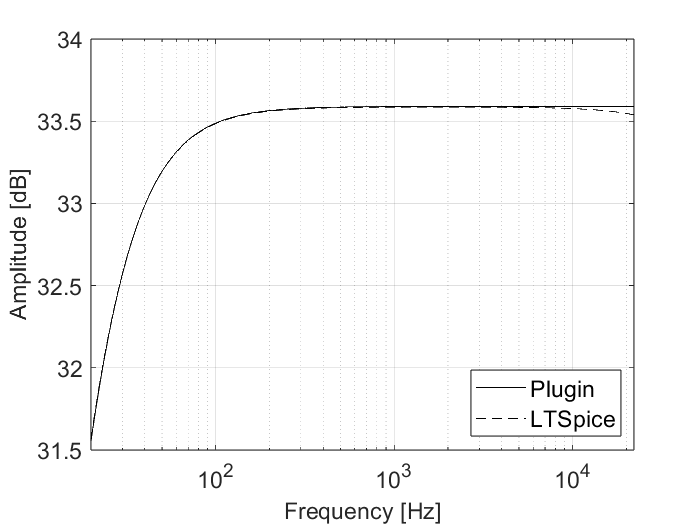
\includegraphics[scale=0.5]{figures/stage8ac.png}
    \caption{Az erősítő kimenő fokozatának áramköre}
\end{figure}
Az átvitelnél a nagy frekvenciáknál valószínűleg azért látható különbség az LTSpice szimuláció és az én megvalósításom között, mert az LTSpice nem ideális műveleti erősítő modellt használ, hanem ilyen nagy erősítéseknél már frekvenciafüggő az átvitele. 

